\documentclass[tikz]{standalone}
\usepackage{tikz,amsmath}
\usetikzlibrary{shapes}
\begin{document}
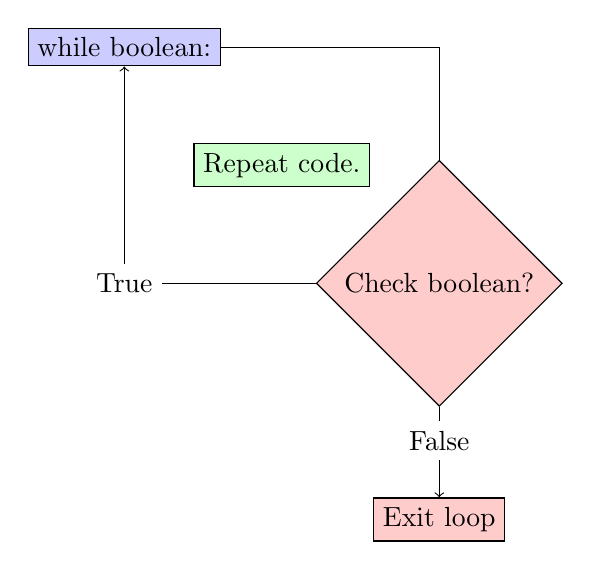
\begin{tikzpicture}
    \node (A) [rectangle, fill=blue!20, draw] at (0, 0) {while boolean:};
    \node [rectangle, fill=green!20, draw] at (2, -1.5) {Repeat code.};
    \node (B) [diamond, fill=red!20, draw] at (4, -3) {Check boolean?};
    \node (C) [rectangle] at (0, -3) {True};
    \draw [->] (A) -- (4,0) -- (B) -- (C) -- (A); 
    \node (D) [rectangle] at (4, -5) {False};
    \node (E) [rectangle, fill=red!20, draw] at (4,-6) {Exit loop};
    \draw [->] (B) -- (D) -- (E);
\end{tikzpicture}
\end{document}
